%------------------------------------------%
% Cannabis Data Science
% Saturday Morning Statistics
% Date: 3/5/2022
%------------------------------------------%
\documentclass[xcolor={dvipsnames}]{beamer}
\hypersetup{pdfpagemode = FullScreen}
\mode<presentation>{
  \usetheme{Boadilla}
  \usecolortheme{orchid}
  \usefonttheme{default}
  \setbeamertemplate{navigation symbols}{}
  \setbeamertemplate{caption}[numbered]
}
\setbeamersize{
  text margin left = 0.5in,
  text margin right = 0.5in
}

%------------------------------------------%
% Title
%------------------------------------------%
\author{Cannabis Data Science}
\title[\textbf{Saturday Morning Statistics \#14}]{}
\institute[]{\Large Saturday Morning Statistics \#14}
\date{March \nth{5}, 2022}

%------------------------------------------%
% Packages
%------------------------------------------%
\usepackage[english]{babel}
\usepackage[utf8x]{inputenc}
\usepackage{tikz}
\usepackage{xparse}

%------------------------------------------%
% Colors
%------------------------------------------%
\definecolor{Green}{RGB}{34, 153, 84}
\definecolor{LightGreen}{RGB}{218, 247, 166}
\definecolor{DarkGreen}{RGB}{2, 48, 32}
\definecolor{Orange}{RGB}{255, 87, 51}
\definecolor{DarkOrange}{RGB}{199, 0, 57}
\definecolor{Yellow}{RGB}{255, 195, 0}

%------------------------------------------%
% Theme
%------------------------------------------%
\setbeamercolor*{palette primary}{bg=LightGreen, fg=DarkGreen}
\setbeamercolor*{palette secondary}{bg=LightGreen, fg=DarkGreen}
\setbeamercolor*{palette tertiary}{bg=LightGreen, fg=DarkGreen}

%------------------------------------------%
% Packages
%------------------------------------------%
\usepackage{amsmath}
\renewcommand*\footnoterule{} % No separating line on footnote.
\usepackage{mathtools} % For annotating equations.
\usepackage{hhline} % for double bars.
\usepackage[super]{nth} % For formatting 1st, 2nd, 3rd, etc.
\usepackage{graphicx, caption, subcaption}
\usepackage{setspace}

%------------------------------------------%
% Commands
%------------------------------------------%

% Top space.
\newcommand\T{\rule{0pt}{2.5ex}}

% Bottom space.
\newcommand\B{\rule[-1.25ex]{0pt}{0pt}}

% Blocks.
\newenvironment<>{Block}[2][.9\textwidth]
  {\setlength{\textwidth}{#1}
  \begin{actionenv}#3
    \def\insertblocktitle{#2}\par
    \usebeamertemplate{block begin}}
  {\par\usebeamertemplate{block end}
  \end{actionenv}}

% Balls.
\defbeamertemplate{enumerate item}{largeball}
{\begin{pgfpicture}{-1ex}{-0.65ex}{1.5ex}{1.5ex}
\usebeamercolor[fg]{item projected}
{\pgftransformscale{2.5}\pgftext{\Large\pgfuseshading{bigsphere}}}
{\pgftransformshift{\pgfpoint{0pt}{0.5pt}}
\pgftext{\usebeamerfont*{item projected}\small\insertenumlabel}}
\end{pgfpicture}}

% Fancy arrows.
\NewDocumentCommand\UpArrow{O{2.0ex} O{black}}{%
   \mathrel{\tikz[baseline] \draw [->, line width=0.5pt, #2] (0,0) -- ++(0,#1);}} % Fancy up-arrow.
\NewDocumentCommand\DownArrow{O{2.0ex} O{black}}{%
   \mathrel{\tikz[baseline] \draw [<-, line width=0.5pt, #2] (0,0) -- ++(0,#1);}} % Fancy down-arrow.

% Equations with numbers on the left.
\makeatletter
\newcommand{\LeftEqNo}{\let\veqno\@@leqno}
\makeatother

%------------------------------------------%
% Presentation
%------------------------------------------%
\begin{document}

%------------------------------------------%
% Title Page
%------------------------------------------%
\begin{frame}{}
  
\includegraphics[scale=0.33]{images/logo.pdf}
  \vspace*{-2\baselineskip}
  \titlepage
\end{frame}

%------------------------------------------%
% Introduction
%------------------------------------------%
\section{Introduction}
\begin{frame}{}

\vspace*{2\baselineskip}

\begin{center}
\begin{minipage}{.6\textwidth}
\itshape ``Life is good for only two things: doing mathematics and teaching it.'' \\[.25\baselineskip]
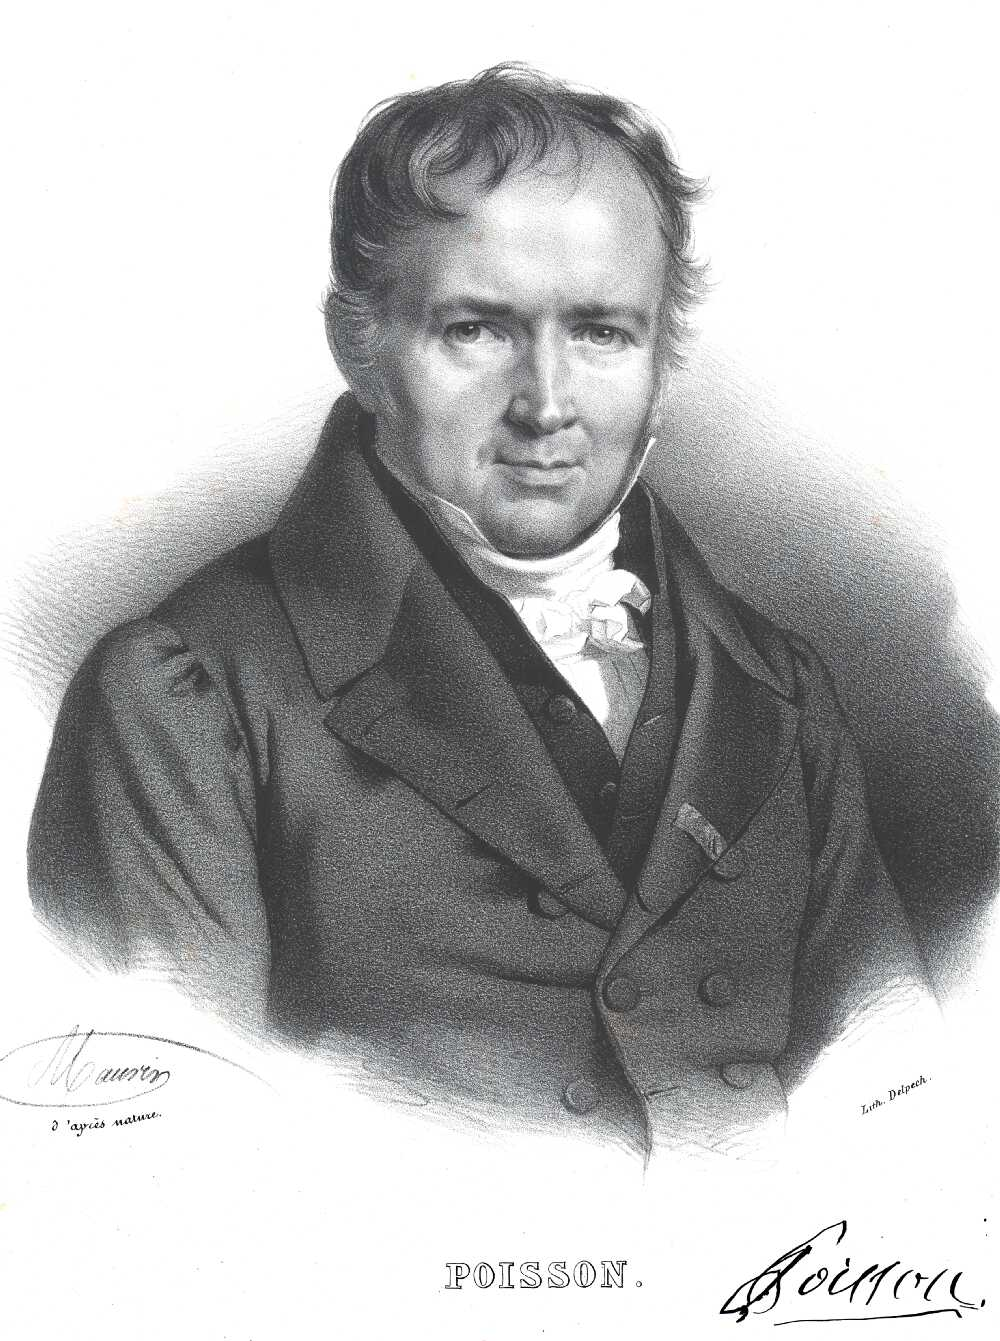
\includegraphics[height=2in]{images/Poisson.jpg}\\[-1.25\baselineskip]
\begin{flushright}
\small -- Sim\'{e}on--Denis Poisson (1781 -- 1840)
\end{flushright}
\end{minipage}
\end{center}

\begin{figure}

\end{figure}

% Methods: Model the number of beverage sales by day (month?) by county in Washington State in relation to the average age of the population.



% TODO: Pharmacology
% https://en.wikipedia.org/wiki/Pharmacology


% TODO: Bioavailability
% https://en.wikipedia.org/wiki/Bioavailability


% TODO: Chimera
% https://en.wikipedia.org/wiki/Chimera_(genetics)


% TODO: Chirality
% https://en.wikipedia.org/wiki/Chirality



\end{frame}

%------------------------------------------%
% History
%------------------------------------------%
\begin{frame}{}

{\large \textbf{A Brief History of Si\'{e}on--Denis Poisson}}\vspace{1\baselineskip}\\

\begin{minipage}{0.6\textwidth}

\vspace{-2\baselineskip}

\begin{itemize}
 
\item Work on integrals, calculus, probability theory.

\vspace{0.25\baselineskip}

\item Published more than 300 works.

\vspace{0.25\baselineskip}

\item Contemporary of

\vspace{0.25\baselineskip}
\begin{itemize}
\item Joseph Louis Lagrange
\vspace{0.25\baselineskip}
\item Pierre--Simon Laplace
\vspace{0.25\baselineskip}
\item Jean Baptiste Joseph Fourier
\end{itemize}
 
\end{itemize}

\end{minipage}\hspace{0.05\textwidth}%
\begin{minipage}{0.33\textwidth}

\begin{figure}
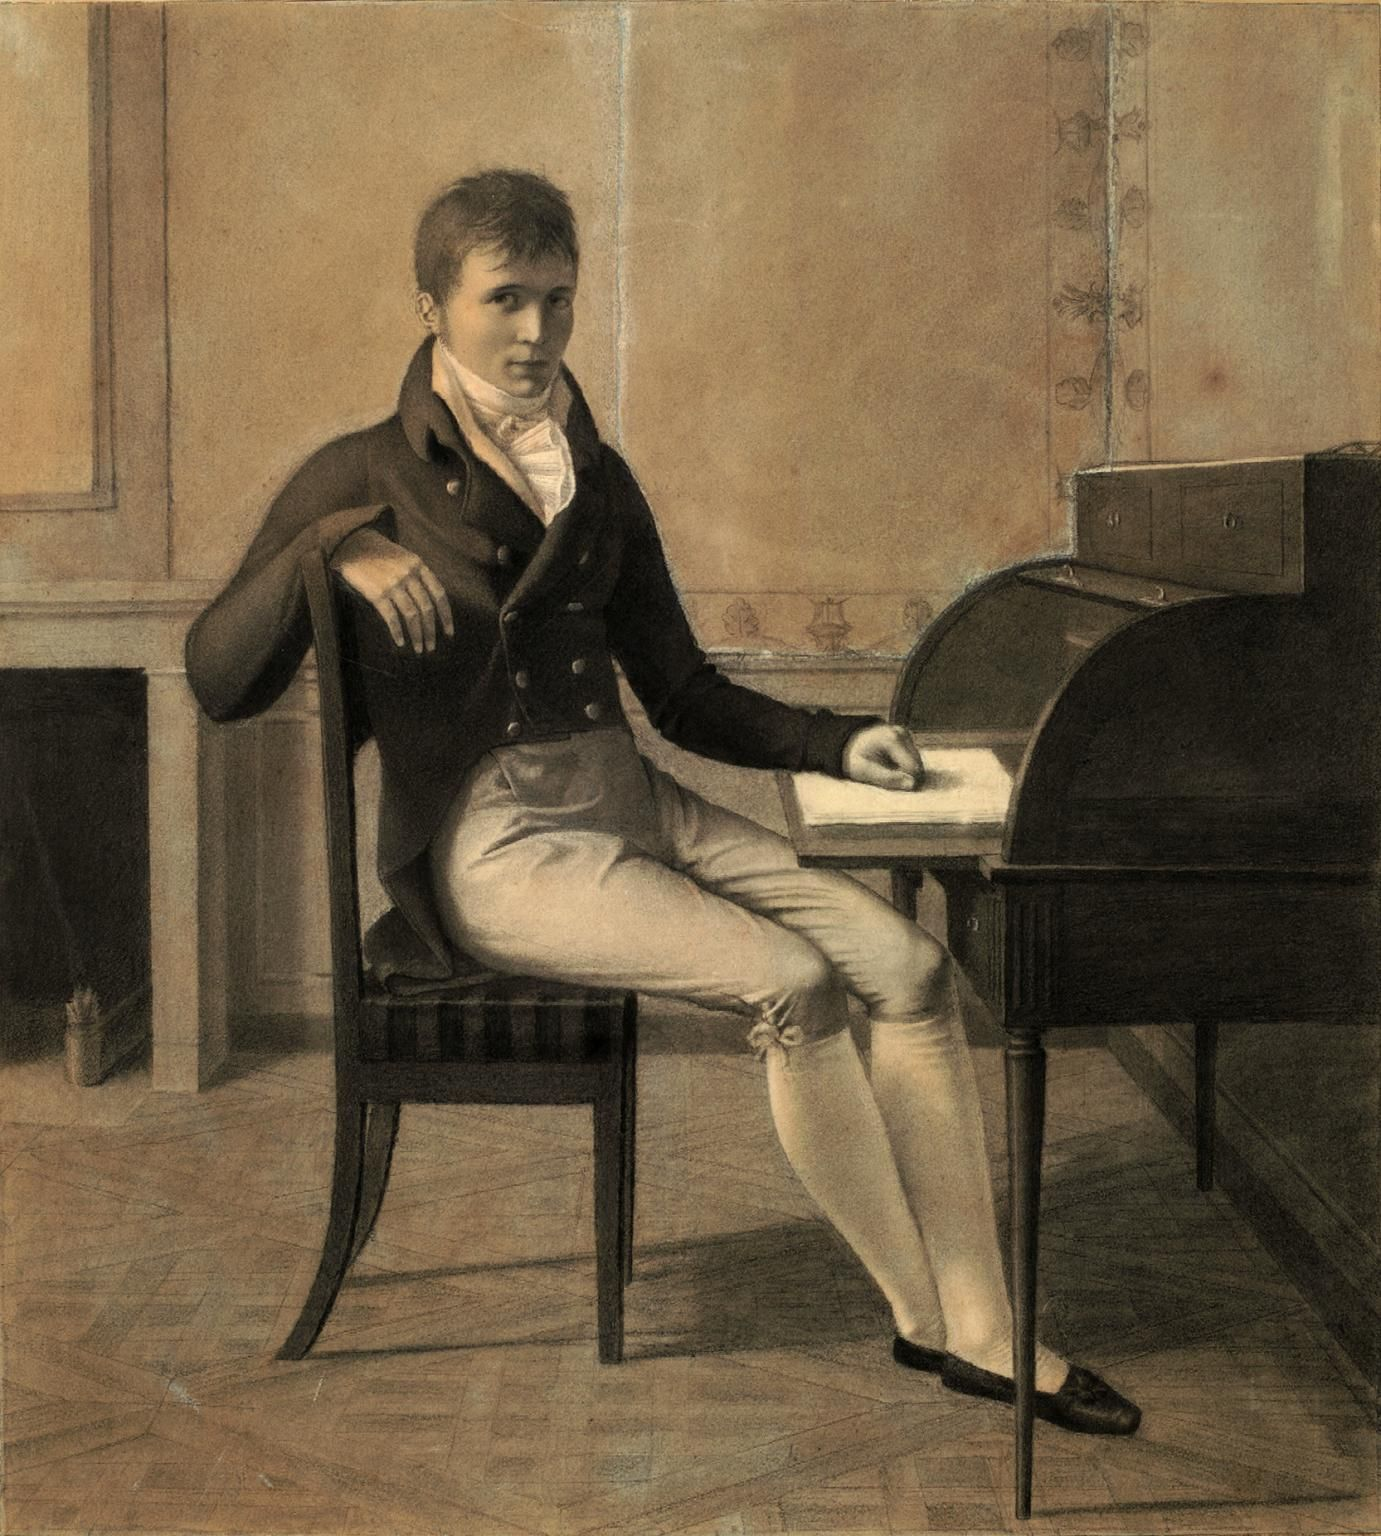
\includegraphics[height=1.5in]{images/Poisson-1804.jpg}
\caption*{%
  \scriptsize
  {Sim\'{e}on--Denis Poisson (1781 -- 1840) in 1804.}
 }
\end{figure}

\end{minipage}


\end{frame}


%------------------------------------------%
% Statistics
%------------------------------------------%
\begin{frame}{}

\vspace{1\baselineskip}
{\large \textbf{The Poisson Distribution}}\vspace{0.75\baselineskip}\\

\begin{minipage}{0.55\textwidth}
\vspace*{-2\baselineskip}
A discrete random variable, $y$, has a Poisson distribution, denoted $$y \sim Po(\lambda),$$ if its probability mass function is

$$
f_{Po}(y|\lambda) = \frac{\lambda^y e^{-\lambda}}{y!},
$$

where $\lambda > 0$ and $y = 0, 1, 2, \dots$

\end{minipage}\hspace{0.05\textwidth}%
\begin{minipage}{0.4\textwidth}

\begin{figure}
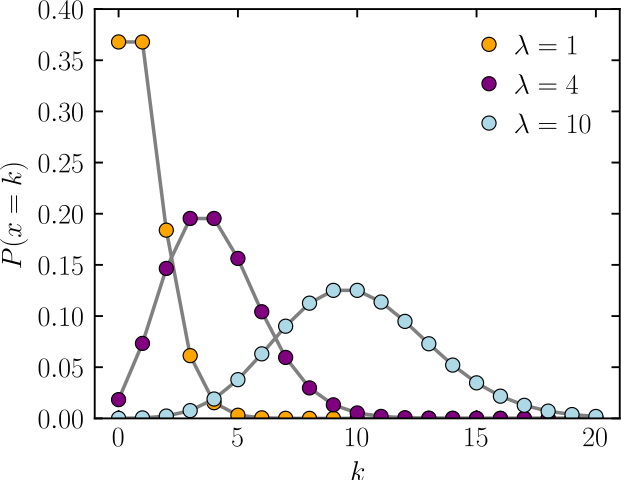
\includegraphics[width=\textwidth]{images/Poisson-distribution.png}
\caption*{
\footnotesize Here, $k$ is the number of occurrences and $\lambda$ is the expected rate of occurrences.\\[0.5\baselineskip]
\tiny Credit: Skbkekas, License: https://creativecommons.org/licenses/by/3.0\\
No changes were made to the figure.
}
\end{figure}

\end{minipage}

\vspace*{0.74\baselineskip}
{\footnotesize
{\bfseries Fun fact}: The mean and variance of the Poisson distribution are equal to the expected rate of occurrences

\vspace{-1.5\baselineskip}
\begin{align*}
E(Y) &= \lambda \\
Var(Y) &= \lambda \\
\end{align*}
}


\end{frame}


%------------------------------------------%
% Models
%------------------------------------------%
\section{Modeling Count Data}
\begin{frame}{}

{\large \textbf{Modeling Discrete Data}}\vspace{0.5\baselineskip}\\

\begin{itemize}

\item The {\bfseries Poisson distribution} is used to model \underline{discrete data} arising from \underline{continuous trials}.

\vspace{1\baselineskip}

\item The {\bfseries binomial distribution} is used to model \underline{discrete trials}.

\vspace{0.75\baselineskip}

% Figure of Poisson, binomial, and normal distribution
\begin{figure}
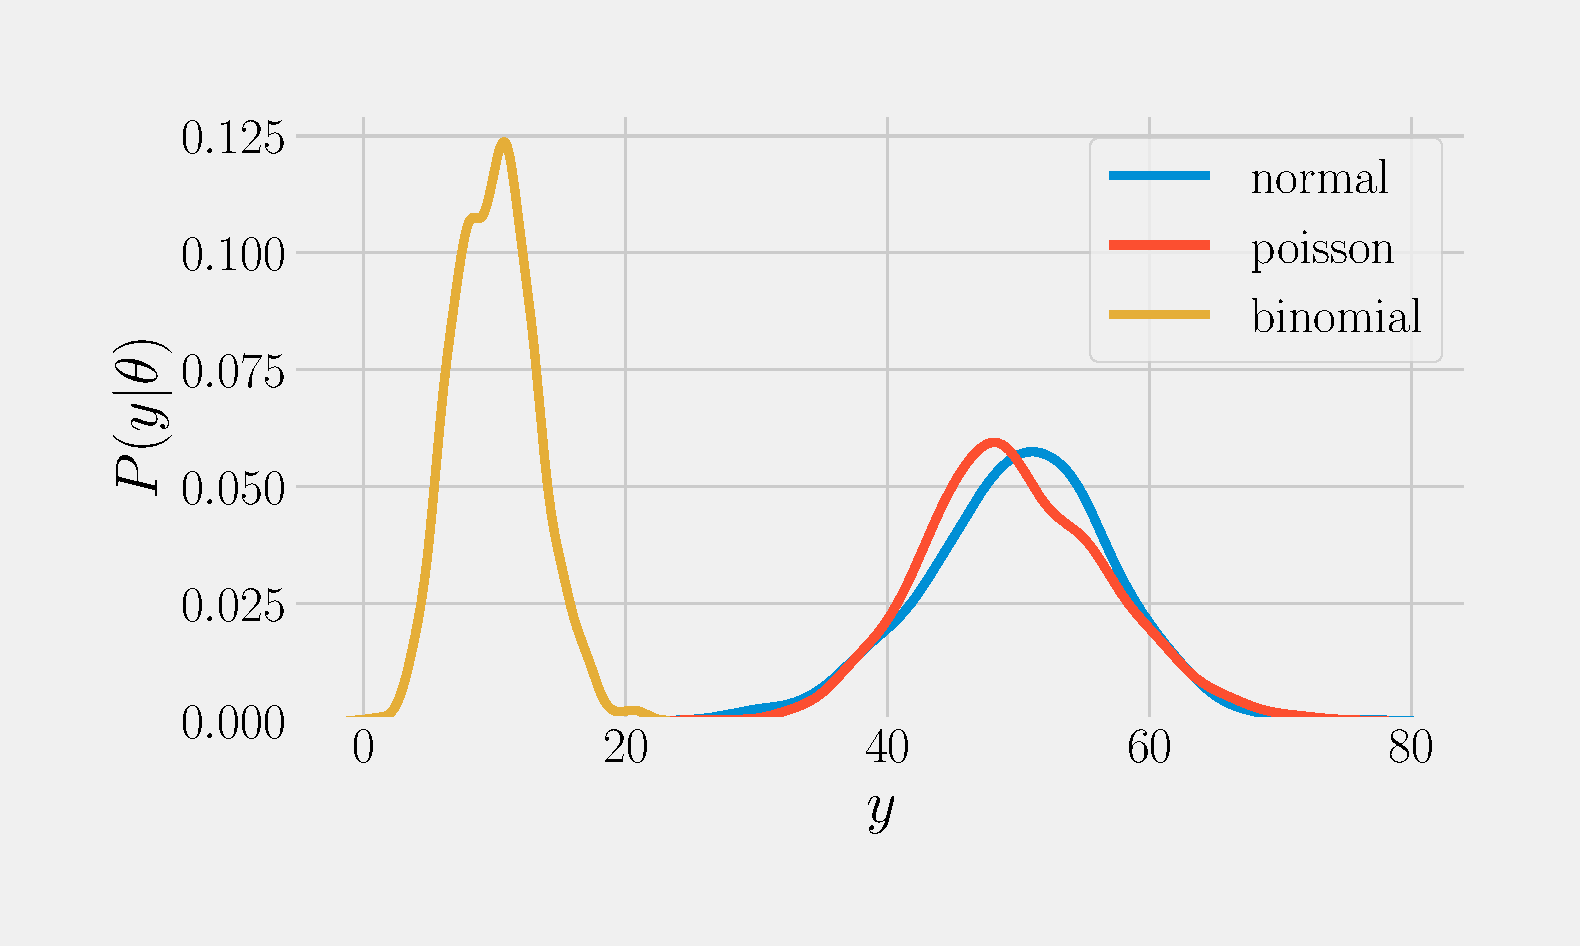
\includegraphics[width=0.65\textwidth]{images/poisson_normal_binomial.pdf}
\end{figure}


\end{itemize}

\vspace{0.25\baselineskip}

{\footnotesize
{\bfseries Fun fact:} Given certain parameters, the {\bfseries binomial distribution} and {\bfseries Poisson distribution} approximate a {\bfseries normal distribution}.
}

% TODO: Plot normal, Poisson, and binomial distributions.

% Normal Distribution
%\begin{minipage}{.45\textwidth}
%\begin{figure}
%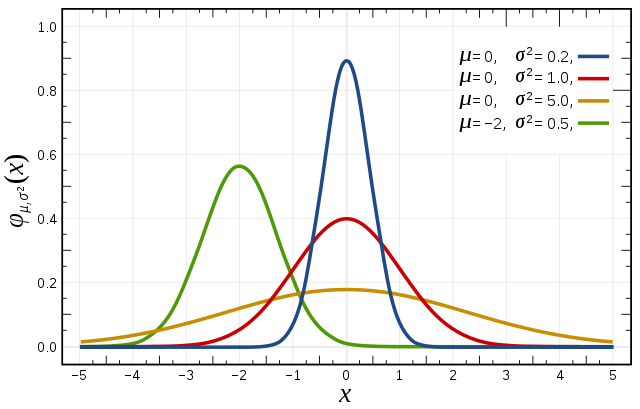
\includegraphics[height=1.1in]{images/normal-distribution.png}
%\caption*{%
%  \scriptsize
%  {\bfseries Normal Distribution}\\[.5\baselineskip]
%  Notation: $\mathcal{N}(\mu, \sigma^2)$\\[.5\baselineskip]
%  Parameters: mean $\mu \in \mathbb{R}$, \\variance $\sigma^2 \in \mathbb{R}_{>0}$\\[.5\baselineskip]
%  PDF:$p(x | \mu, \sigma^2) = \frac{1}{\sigma\sqrt{2\pi}}\text{exp}\left[ -\frac{1}{2}\left( \frac{x - \mu}{\sigma} \right)^2 \right]
%$
%}
%\end{figure}
%\end{minipage}\hspace{.05\textwidth}%
%% Gamma Distribution
%\begin{minipage}{.45\textwidth}
%\begin{figure}
%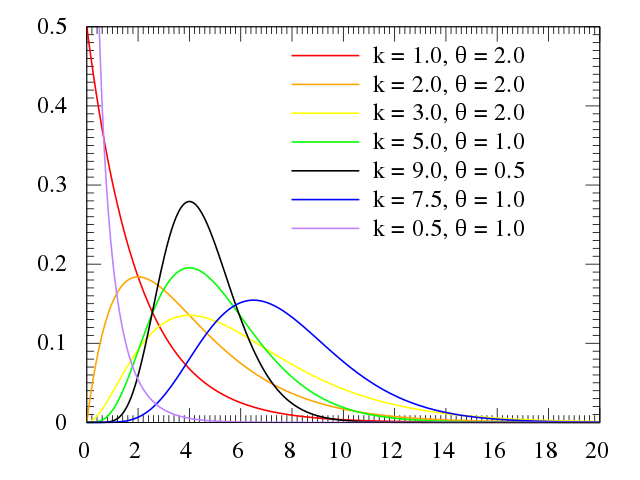
\includegraphics[height=1.1in]{images/gamma-distribution.png}
%\caption*{%
%  \scriptsize
%  {\bfseries Gamma Distribution}\\[.5\baselineskip]
%  Notation: $Y \sim G(\alpha, \beta)$\\[.5\baselineskip]
%  Parameters: shape $\alpha > 0$, rate $\beta > 0$\\[.5\baselineskip]
%  PDF:$
%  f_\gamma(y | \alpha, \beta ) \equiv   \begin{cases}
%    (\beta^\alpha \Gamma(\alpha))^{-1} y^{\alpha - 1}\text{exp}(-y /\beta)& \text{if } 0 < y < \infty \\
%    0 & \text{otherwise.}
%\end{cases}$
%}
%\end{figure}
%\end{minipage}

\vfill

%{\tiny Gamma Distribution figure credit \\ Authors: MarkSweep and Cburnett \\ License: https://creativecommons.org/licenses/by-sa/3.0/deed.en\\[-1\baselineskip] No changes were made to the figure.}

\end{frame}


%------------------------------------------%
% Question of the day
%------------------------------------------%
\begin{frame}{}

\begin{center}
\begin{minipage}{.9\linewidth}
\begin{Block}{Question of the Day: Beverage Preferences}

\vspace{.5\baselineskip}
\begin{itemize}
\item Does age or any other factor affect people's preferences for liquid edibles?
\end{itemize}

\vspace{.5\baselineskip}

\end{Block}
\end{minipage}
\end{center}

% TODO: Beverage image
\begin{center}
\begin{minipage}{0.5\textwidth}
\begin{figure}
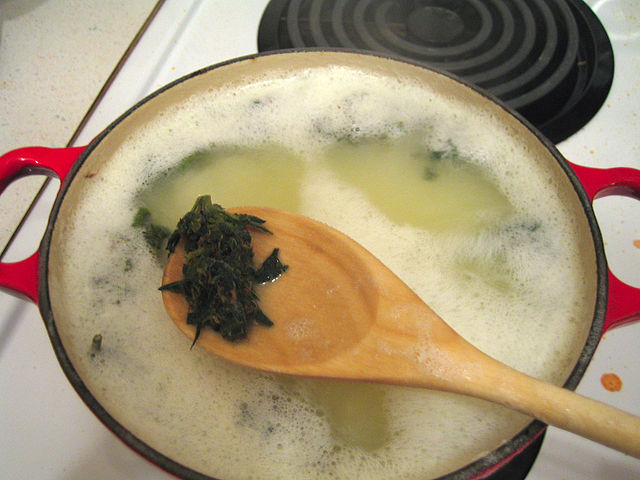
\includegraphics[width=\textwidth]{images/cannabutter.jpg}
\caption*{\footnotesize Homemade cannabutter that can be used as an intermediary product. For example, in a cup of {\itshape butter coffee}.}
\end{figure}
\end{minipage}
\end{center}


\end{frame}
% Question of the day: Does age affect people's preference for liquid edibles?

%------------------------------------------%
% Takeaway
%------------------------------------------%
\section{Takeaway}
\begin{frame}{}

\begin{center}
\begin{minipage}{3.85in}

% Thank you.
\begin{center}

\includegraphics[width=.25in]{images/prayer.png} {\Large \textbf{Thank you for coming.}}\\
\end{center}
\vspace*{0.5\baselineskip}

% Re-cap the lesson of the week.
\begin{center}
\begin{minipage}{\linewidth}
\begin{Block}{Lessons of the Day}

\vspace{0.5\baselineskip}

\begin{itemize}

\item Have the right model for the task at hand.

\vspace{0.5\baselineskip}

\item We can get a good pulse of cannabis markets with count-based models.

\vspace{0.5\baselineskip}

\end{itemize}

\end{Block}
\end{minipage}
\end{center}

\vspace*{2\baselineskip}

%{\bfseries References}\\[-0.75\baselineskip]
%
%Bayesian Econometric Methods,  Koop, Poirier, and Tobias (2007).

\end{minipage}
\end{center}

\end{frame}


%------------------------------------------%
% End
%------------------------------------------%
\end{document}
